\chapter{Context-aware recommendation}

\section{Location-aware recommendation}
\begin{itemize}
\item Users, interactions and occasionally items have locations.
\item Data with location information is rich.
\item We can make better recommendtaion using this information.
\end{itemize}

\section{Data with location information}
\begin{itemize}
\item What is Twitter?
  \begin{itemize}
    \item User, hashtag, tweet, mention, retweet, follow.
  \end{itemize}
\item Twitter has public API, which gave us opportunity to get rich twitter
  data with coordinates.
\item ELTE collected the data
\end{itemize}

\subsection{Data parsing and cleansing}
The dataset we examine was gathered between February 1 2012 and January 1 2013
through Twitter's streamingAPI and was restricted to geo-tagged tweets. The
dataset consists of more that 1.4 billion tweets, including the original
tweets of around 30 million retweets. In the base data set each tweet is a
JSON document. We parsed the JSON files, and created CSV files that archive
only the relevant information for us. Duplicated or unparseable lines have been
removed. In case of a retweet, the JSON document contains informations on the
original root tweet, that we added to the set of tweets. Because of the
simplicity of CSV, the data may have informationredundancy, but it allows us
to make more robust andreusable codes. Since we wish to work with entities and
attributes (likehashtags and @-mentions) using their timestamp, we organised
the different entities into different files and grouped and sorted them
accordingly. By reason of the size of the data, we run our parser applications
in parallel and after merge the results. That is how we get our main timeline
es, for instance hashtag, url, mention, usertimelines. All timelines contain
not only timestamps and entities, but also the geographical information of the
tweets.
\begin{enumerate}
\item GADM tree
\end{enumerate}
\subsection{Statistics}

\section{Using matrix factorization for hashtag recommendation}
\begin{enumerate}
\item We would have liked to predict a the users first hashtag adoptation
\item We used item and user factors to compute the scores
\item We used NDCG to evaluate our predictions 
\end{enumerate}


\section{Using recency and popularity functions for hashtag recommendation}

\section{Music recommendation}

\begin{itemize}
\item Relevance the music recommendation
\item Music related data has several interesting features
  \begin{itemize}
  \item genre
  \item tag
  \item playlist
  \item artist
  \item album
  \end{itemize}
\item Music sessions are highly temporal behavings, that's why we use online
  algorithms
\item nmusic
\item streaming feasibility
\end{itemize}

\subsection{30M music data}
\begin{figure}[h]
\centering
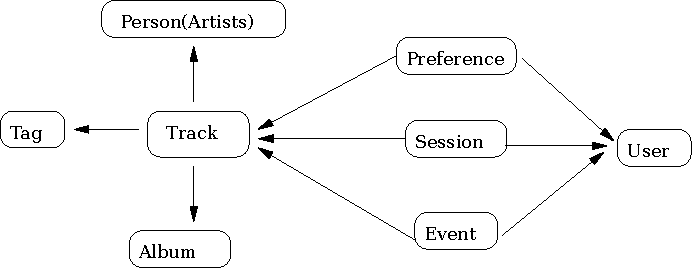
\includegraphics[scale=1]{tex/pic/30m_data_structure.pdf}
\end{figure}


\subsection{Attribute based recommendation}
\begin{itemize}
\item We would have liked to use the track features
\item Our basic modell is $r_t = q_u \sum_{j\in\mathcal{F}_t}p_j$,
  where $\mathcal{F}_t$ is the feature set of the track $t$
\end{itemize}

\subsection{Hiden markov?!?}
